\documentclass{article}
\usepackage[preprint]{neurips_2024} % clean preprint style
\usepackage[utf8]{inputenc}
\usepackage[T1]{fontenc}
\usepackage{hyperref}
\usepackage{url}
\usepackage{booktabs}
\usepackage{amsmath}
\usepackage{amssymb}
\usepackage{graphicx}
\usepackage{microtype}

\title{Hebbian Associative Memory for State Space Models}

\author{
  Jeff Guan \\
  Independent \\
  \texttt{jeff@jeffguan.com}
}

\begin{document}

\maketitle

\begin{abstract}
We augment Mamba, a state space model, with a per-layer Hebbian associative memory matrix $W \in \mathbb{R}^{d \times d}$. $W$ accumulates key-value associations via outer-product updates with exponential decay, and injects retrieved content into the residual stream. The mechanism adds 32 lines of code, keeps the training objective, uses $O(d^2)$ memory constant in sequence length, and admits a parallel scan formulation analogous to Mamba's own recurrence, making it nearly drop-in. On PG-19 prose, an 18M-parameter (P) memory model outperforms P-matched baselines (deeper and wider) by 0.05--0.11 nats [TODO: re-evaluate context length scaling claim]. On Python code, the effect is dramatically larger: the memory model achieves a final validation loss 0.94 nats below a P-matched baseline, surpassing the baseline's best-ever performance after only ${\sim}$800K training tokens out of 6M. Although trained at 2K tokens, at 16K evaluation windows the gap expands to over 1.0 nats around 8K as $W$ accumulates file-level associations at test time. Code identifiers are key-value pairs bound once and queried repeatedly, exactly what $W$ implements. The benefit scales across sequence length, training compute, and data complexity [TODO: confirm with 100M results]. The linearity of the update rule, with constant memory cost, has potential implications for image and video sequences where long-range entity persistence is similarly associative.
\end{abstract}

\section{Introduction}

SSMs (e.g.\ Mamba \citep{gu2023mamba}) achieve linear-time sequence modeling by compressing history into a fixed-size recurrent state, fundamentally lossy. Transformers avoid this with a full-context KV cache, but at $O(T^2)$ time and $O(T)$ memory.

The question we address is simple: can we give an SSM a persistent associative memory without the quadratic cost of attention?

We answer yes with a simple mechanism. At each Mamba layer, we maintain a matrix $W \in \mathbb{R}^{d \times d}$ that accumulates associations between consecutive hidden states via Hebbian outer-product updates:
\begin{equation}
    W_t \leftarrow \gamma W_{t-1} + \text{proj}_\text{write}(r_t) \otimes r_{t-1}
\end{equation}
where $r_t$ is the residual-stream vector at step $t$ and $\gamma = \sigma(\lambda)$ is a learned scalar decay. At each step, the model reads from $W$ and injects the result into the residual stream:
\begin{equation}
    r_t \leftarrow r_t + \alpha \cdot \text{proj}_\text{read}(W_t \cdot r_t)
\end{equation}
with $\alpha = 0.03$ fixed. The learned parameters are a scalar $\lambda$ and two $d \times d$ projection matrices. $W$ itself is recurrent state, not a parameter; initialized to zero at the start of each sequence and accumulating during the forward pass.

This update rule is a linear recurrence in $W$, admitting a parallel scan formulation for training and an $O(d^2)$ per-step recurrent form for inference. Unlike attention, memory cost is constant in sequence length.

\paragraph{Why Mamba, not Transformers.}
Transformers have lossless KV-cache memory within the context window --- $W$ has no gap to fill. Mamba's lossy recurrent state creates that gap; the mechanisms are complementary: Mamba handles local context efficiently, $W$ handles long-range associations persistently.

\paragraph{Why code.}
Code is almost entirely associative recall: every identifier is defined once and referenced many times. A Mamba baseline must track all variable bindings through $d_\text{state} = 16$ recurrent dimensions; $W$ stores them directly in a $d \times d$ matrix with $O(\sqrt{d})$ effective capacity scaling.

\paragraph{Contributions.}
\begin{itemize}
    \item A minimal Hebbian memory mechanism for SSMs: one matrix, one decay, one outer product per step.
    \item Demonstration that $W$ learns useful associations under standard language modeling training with no resets or auxiliary objectives.
    \item On prose (PG-19): $+0.05$ nats over a P-matched deep baseline and $+0.11$ nats over wide (2.477 vs.\ 2.527 vs.\ 2.589 val loss), gap growing with context length beyond training length. All models are substantially undertrained at 6M tokens; the gap is still widening at the end of training.
    \item On code (Python): a 0.94 nat improvement over a P-matched baseline at 18M parameters. The memory model surpasses the baseline's final performance after ${\sim}$800K training tokens. At 16K tokens (test time), the per-segment gap exceeds 1.0 nats.
    \item Evidence that the benefit scales along three axes simultaneously: sequence length, training compute, and data complexity (prose to code).
\end{itemize}

\section{Method}

\paragraph{Setup.}
Let $r_t \in \mathbb{R}^d$ denote the residual-stream vector at position $t$, after the Mamba block at a given layer. Each layer maintains an associative memory matrix $W \in \mathbb{R}^{d \times d}$, initialized to zero at the start of each sequence. $W$ is recurrent state, not a learned parameter.

\paragraph{Write.}
After each token, $W$ is updated via a Hebbian outer-product rule with exponential decay:
\begin{equation}
    W_t \leftarrow \gamma W_{t-1} + \text{proj}_\text{write}(r_t) \otimes r_{t-1}
\end{equation}
The key written at step $t$ is $r_{t-1}$ (the previous residual state); the value is $\text{proj}_\text{write}(r_t)$ (the current residual, projected). $\gamma = \sigma(\lambda) \in (0,1)$ is a learned scalar decay controlling memory timescale; associations older than ${\sim}1/(1-\gamma)$ steps are exponentially suppressed.

\paragraph{Read.}
The model retrieves from $W$ by querying with the current state and injecting the result:
\begin{equation}
    r_t \leftarrow r_t + \alpha \cdot \text{proj}_\text{read}(W_t \cdot r_t)
\end{equation}
$W_t \cdot r_t$ computes the inner product between $r_t$ and all previously written keys, returning the corresponding weighted sum of values. $\alpha = 0.03$ is fixed.

\paragraph{Parallel form (training).}
Unrolling the recurrence, all reads across a sequence of length $T$ can be computed as:
\begin{equation}
    \text{reads} = (M \odot S)\, V
\end{equation}
where $S[t,s] = r_t^\top r_{s-1}$ is the $T \times T$ similarity matrix, $M[t,s] = \gamma^{t-1-s} \cdot \mathbf{1}[s < t]$ is a causal exponential decay mask, and $V[s] = \text{proj}_\text{write}(r_s)$. This is analogous to unnormalized causal attention with a fixed decay kernel, at $O(T^2 d)$ time and $O(T^2)$ memory.

\paragraph{Recurrent form (inference).}
$W$ is updated one step at a time at $O(d^2)$ per step and $O(d^2)$ memory, constant in sequence length.

\paragraph{Parameters.}
Each layer adds scalar $\lambda$, $\text{proj}_\text{write} \in \mathbb{R}^{d \times d}$, and $\text{proj}_\text{read} \in \mathbb{R}^{d \times d}$ --- roughly $2d^2$ parameters per layer, or ${\sim}0.5$M at $d=512$.

\paragraph{Design choices.}
\begin{itemize}
    \item \textit{Fixed $\alpha$}: A learned injection scale risks instability early in training when $W$ contains noise. $\alpha = 0.03$ was set by hand and not tuned.
    \item \textit{Separate $\text{proj}_\text{write}$ / $\text{proj}_\text{read}$}: Allows the model to learn different subspaces for writing and reading, analogous to separate key and value projections in attention. $r_t$ is used directly as the query.
    \item \textit{No auxiliary objectives}: $W$ trains end-to-end under the standard language modeling loss. The model learns to use $W$ because it is useful for next-token prediction.
    \item \textit{Per-layer $W$}: Each layer maintains an independent matrix, allowing different layers to specialize in association type and timescale via their learned $\gamma$.
\end{itemize}

\section{Experiments and Results}

All models use AdamW with a cosine LR schedule, batch size $B=2$, sequence length $T=2048$, and ${\sim}$6M training tokens unless otherwise noted. All baselines are parameter-matched to the memory model.

\subsection{Synthetic KV Recall}

We train a small memory model ($d=128$, 4 layers) on a synthetic task: a sequence of 32 key-value pairs followed by 32 queries, where the Mamba recurrent state is reset between store and query phases so any successful recall must pass through $W$.

The model achieves near-perfect recall up to the training distribution (100\% at ${\leq}16$ pairs, 99.8\% at 32) and 96\% at 64 pairs ($2\times$ training count). Without $W$, the reset Mamba state has no mechanism to carry associations, giving chance performance ($1/16 \approx 6.2\%$).

\subsection{Memory Capacity}

We sweep the number of key-value pairs at test time (256 possible keys, 16 values, same trained model):

\begin{table}[h]
\centering
\begin{tabular}{rr}
\toprule
Pairs & Accuracy \\
\midrule
4--16 & 100.0\% \\
32    & 99.8\%  \\
64    & 96.0\%  \\
128   & 55.7\%  \\
256   & 18.8\%  \\
\bottomrule
\end{tabular}
\end{table}

Naive random-key theory predicts $\text{SNR} \approx \sqrt{d/k} \approx 1.4$ at $k=64$, corresponding to ${\sim}50$--70\% recall. The model achieves 96\%, indicating learned projections structure keys to reduce interference. At 256 pairs, 18.8\% accuracy corresponds to ${\sim}$48 correct, or ${\sim}$12 per layer across 4 independent $W$ matrices --- within single-matrix capacity.

\subsection{Param-Matched Baselines on Prose (PG-19)}

We compare three models on PG-19: an 8-layer memory model ($d=512$, 18.0M params), a 10-layer deep baseline ($d=512$, 17.2M), and an 8-layer wide baseline ($d=576$, 17.4M). All trained identically at $B=2$, $T=2048$, 1465 steps (${\sim}$6M tokens).

\begin{table}[h]
\centering
\begin{tabular}{lrr}
\toprule
Model & Val Loss & PPL \\
\midrule
Memory ($d=512$, 8L) & 2.477 & 11.91 \\
Deep ($d=512$, 10L)  & 2.527 & 12.51 \\
Wide ($d=576$, 8L)   & 2.589 & 13.32 \\
\bottomrule
\end{tabular}
\end{table}

The memory model outperforms both parameter-matched baselines. The memory model is also ${\sim}$500ms faster per training step than the deep baseline (dense BMMs vs.\ Mamba's parallel scan), so the gap is larger at iso-FLOPs.

Training dynamics are shown in Figure~\ref{fig:prose_training}. The gap over the wide baseline grows throughout training (Table~\ref{tab:prose_dynamics}), indicating all models are substantially undertrained at 6M tokens.

\begin{table}[h]
\centering
\caption{Val loss (nats) on PG-19 at training checkpoints.}
\label{tab:prose_dynamics}
\begin{tabular}{lrrr}
\toprule
Tokens & Memory & Deep & Wide \\
\midrule
2M & 2.806 & 2.854 & 2.838 \\
4M & 2.561 & 2.613 & 2.625 \\
6M & 2.477 & 2.527 & 2.589 \\
\bottomrule
\end{tabular}
\end{table}

\begin{figure}[h]
\centering
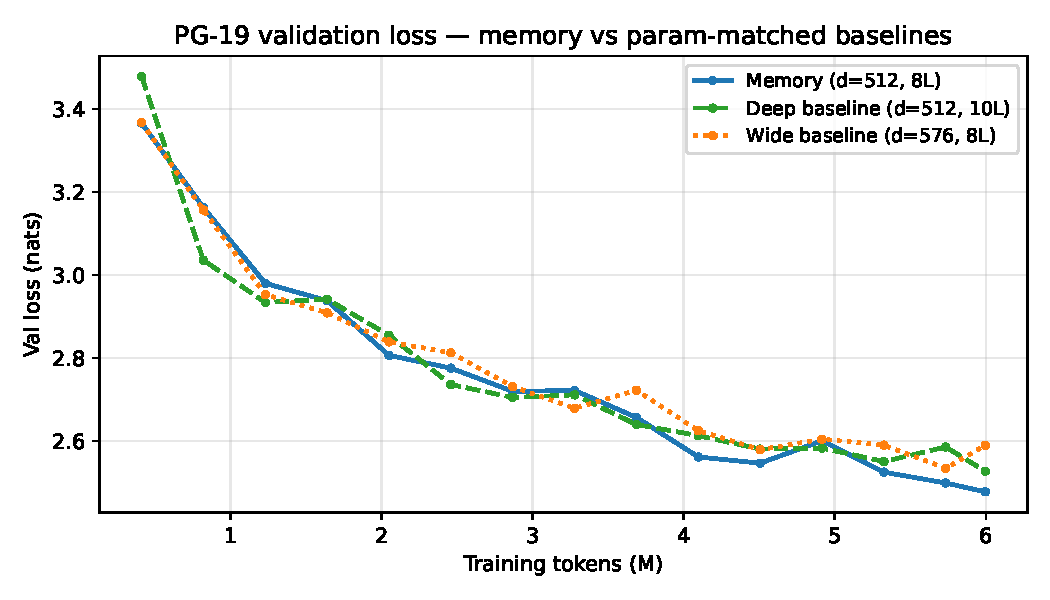
\includegraphics[width=0.85\textwidth]{figures/prose_training.pdf}
\caption{PG-19 val loss over training. The gap over the wide baseline is still widening at 6M tokens.}
\label{fig:prose_training}
\end{figure}

\paragraph{Context length scaling.}
Evaluating the trained models at longer contexts with no fine-tuning (memory vs.\ wide baseline):

\begin{table}[h]
\centering
\begin{tabular}{lrrr}
\toprule
Eval length & Memory & Wide & Gap \\
\midrule
16K (8$\times$ train)  & 2.482 & 2.500 & $+$0.019 \\
64K (32$\times$ train) & 2.484 & 2.512 & $+$0.028 \\
\bottomrule
\end{tabular}
\end{table}

The gap grows with context length as $W$ accumulates associations. Both models generalise far beyond their 2K training length with no degradation.

\paragraph{W ablation.}
To confirm that $W$ itself (not just the additional parameters) drives the improvement, we compare two inference passes on the trained code model: normal ($W$ updating each step) vs.\ frozen ($W$ reset to its pre-step value, so it never accumulates). Over 8 random 8K-token windows:

\begin{table}[h]
\centering
\begin{tabular}{lrr}
\toprule
 & Val Loss & vs.\ updating \\
\midrule
$W$ updating (normal) & 2.019 & --- \\
$W$ frozen            & 2.914 & $+$0.895 \\
\bottomrule
\end{tabular}
\end{table}

Freezing $W$ costs 0.895 nats --- nearly equal to the full memory-vs-baseline gap of 0.939. The improvement comes from $W$, not from the extra parameters. The delta is large from position 0 and consistent throughout the sequence, indicating $W$ provides useful associations immediately. All 8 layers converge to $\gamma \approx 0.99$, giving an effective memory window of ${\sim}$100--150 steps.

\subsection{Context Length Scaling on Prose}

We evaluate the trained prose models at longer contexts with no fine-tuning (memory vs.\ wide baseline, averaged over 8 random windows): [TODO: increase window count --- gap is small (+0.019) and per-segment variance is high; 8 windows may be insufficient for significance]

\begin{table}[h]
\centering
\begin{tabular}{lrrr}
\toprule
Eval length & Memory & Wide & Gap \\
\midrule
16K (8$\times$ train) & 2.482 & 2.500 & $+$0.019 \\
\bottomrule
\end{tabular}
\end{table}

Both models generalise far beyond their 2K training length. The memory advantage is positive and consistent with $W$ accumulating associations over longer sequences. The effect is modest on prose; the gap becomes dramatically larger on code (Section~\ref{sec:code}).

\subsection{Code (Headline Result)}
\label{sec:code}

We train on Python files from codeparrot/codeparrot-clean (files $\geq$4096 chars), using a 512-vocab BPE tokenizer yielding ${\sim}$16M training tokens. The memory model is 8-layer (18.0M params) and the baseline is the 10-layer deep model (17.2M params), trained identically.

\begin{table}[h]
\centering
\caption{Final val loss on Python code after 6M training tokens.}
\begin{tabular}{lrrr}
\toprule
Model & Val Loss & BPB & PPL \\
\midrule
Memory (d=512, 8L) & 1.848 & 1.33 & 6.35  \\
Deep (d=512, 10L)  & 2.787 & 2.01 & 16.24 \\
Gap                & $+$0.939 & $+$0.68 & \\
\bottomrule
\end{tabular}
\end{table}

The gap is $10\times$ larger than on prose. Training curves are shown in Figure~\ref{fig:code_training}; the memory model surpasses the baseline's final val loss by step 200 (${\sim}$800K tokens, 14\% of total training).

\begin{table}[h]
\centering
\caption{Code val loss during training.}
\begin{tabular}{lrrr}
\toprule
Tokens & Memory & Deep & Gap \\
\midrule
0.4M & 3.207 & 3.782 & $+$0.575 \\
0.8M & 2.739 & 3.329 & $+$0.590 \\
2.0M & 2.195 & 3.215 & $+$1.021 \\
4.1M & 2.024 & 2.571 & $+$0.547 \\
6.0M & 1.848 & 2.787 & $+$0.939 \\
\bottomrule
\end{tabular}
\end{table}

\begin{figure}[h]
\centering
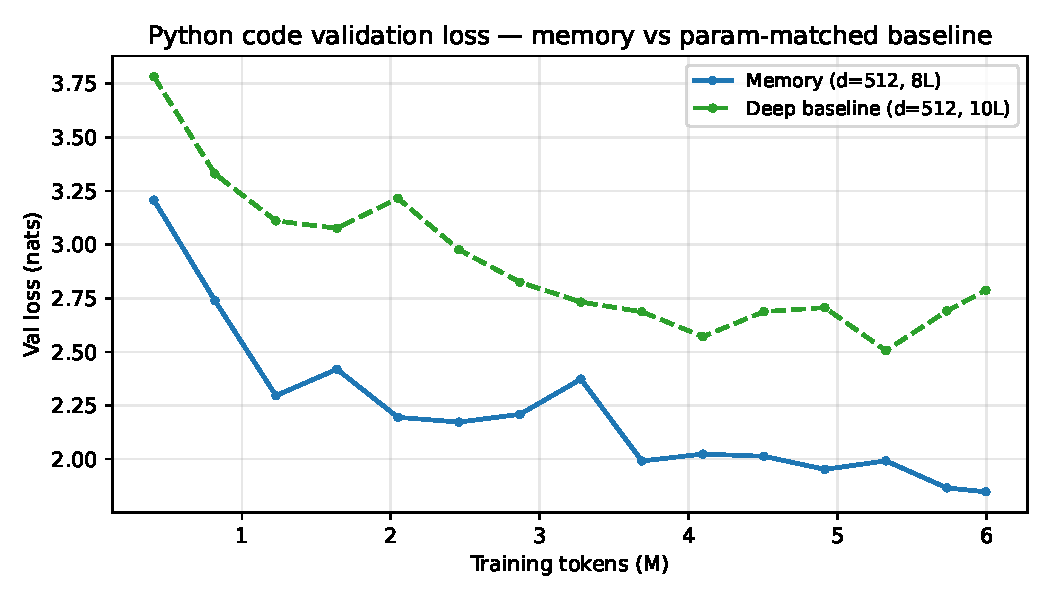
\includegraphics[width=0.85\textwidth]{figures/code_training.pdf}
\caption{Python code val loss over training. The memory model surpasses the baseline's final performance by 0.8M tokens.}
\label{fig:code_training}
\end{figure}

\paragraph{Long-context evaluation.}
We evaluate both models on 4 random 16K-token windows (8$\times$ training length) with no fine-tuning, measuring per-segment loss at 1K intervals:

\begin{table}[h]
\centering
\begin{tabular}{lrrr}
\toprule
Segment & Memory & Deep & Gap \\
\midrule
0K--1K   & 2.203 & 2.650 & $+$0.447 \\
2K--3K   & 2.011 & 2.632 & $+$0.622 \\
7K--8K   & 1.631 & 2.698 & $+$1.067 \\
15K--16K & 1.676 & 2.484 & $+$0.809 \\
\midrule
Overall  & 1.912 & 2.658 & $+$0.746 \\
\bottomrule
\end{tabular}
\end{table}

The per-segment gap grows from $+$0.447 at 0--1K to $+$1.067 at 7--8K as $W$ accumulates file-level associations. Identifiers referenced late in a file were bound early; $W$ retrieves them directly while the baseline must retain all bindings through its recurrent state.

\end{document}
